\documentclass[]{article}
\usepackage[left=1in,top=1in,right=1in,bottom=1in]{geometry}


%%%% more monte %%%%
% thispagestyle{empty}
% https://stackoverflow.com/questions/2166557/how-to-hide-the-page-number-in-latex-on-first-page-of-a-chapter
\usepackage{color}
\usepackage[table]{xcolor} % are they using color?

\definecolor{WSU.crimson}{HTML}{981e32}
\definecolor{WSU.gray}{HTML}{5e6a71}

\definecolor{shadecolor}{RGB}{248,248,248}
\definecolor{WSU.crimson}{RGB}{152,30,50} % use http://colors.mshaffer.com to convert from 981e32
\definecolor{WSU.gray}{RGB}{94,106,113}

%%%%%%%%%%%%%%%%%%%%%%%%%%%%

\newcommand*{\authorfont}{\fontfamily{phv}\selectfont}
\usepackage{lmodern}


\usepackage[T1]{fontenc}
  \usepackage[utf8]{inputenc}




\usepackage{abstract}
\renewcommand{\abstractname}{}    % clear the title
\renewcommand{\absnamepos}{empty} % originally center

\renewenvironment{abstract}
 {{%
    \setlength{\leftmargin}{0mm}
    \setlength{\rightmargin}{\leftmargin}%
  }%
  \relax}
 {\endlist}

\makeatletter
\def\@maketitle{%
  \pagestyle{empty}
  \newpage
%  \null
%  \vskip 2em%
%  \begin{center}%
  \let \footnote \thanks
    {\fontsize{18}{20}\selectfont\raggedright  \setlength{\parindent}{0pt} \@title \par}%
}
%\fi
\makeatother






\usepackage{color}
\usepackage{fancyvrb}
\newcommand{\VerbBar}{|}
\newcommand{\VERB}{\Verb[commandchars=\\\{\}]}
\DefineVerbatimEnvironment{Highlighting}{Verbatim}{commandchars=\\\{\}}
% Add ',fontsize=\small' for more characters per line
\usepackage{framed}
\definecolor{shadecolor}{RGB}{248,248,248}
\newenvironment{Shaded}{\begin{snugshade}}{\end{snugshade}}
\newcommand{\AlertTok}[1]{\textcolor[rgb]{0.94,0.16,0.16}{#1}}
\newcommand{\AnnotationTok}[1]{\textcolor[rgb]{0.56,0.35,0.01}{\textbf{\textit{#1}}}}
\newcommand{\AttributeTok}[1]{\textcolor[rgb]{0.77,0.63,0.00}{#1}}
\newcommand{\BaseNTok}[1]{\textcolor[rgb]{0.00,0.00,0.81}{#1}}
\newcommand{\BuiltInTok}[1]{#1}
\newcommand{\CharTok}[1]{\textcolor[rgb]{0.31,0.60,0.02}{#1}}
\newcommand{\CommentTok}[1]{\textcolor[rgb]{0.56,0.35,0.01}{\textit{#1}}}
\newcommand{\CommentVarTok}[1]{\textcolor[rgb]{0.56,0.35,0.01}{\textbf{\textit{#1}}}}
\newcommand{\ConstantTok}[1]{\textcolor[rgb]{0.00,0.00,0.00}{#1}}
\newcommand{\ControlFlowTok}[1]{\textcolor[rgb]{0.13,0.29,0.53}{\textbf{#1}}}
\newcommand{\DataTypeTok}[1]{\textcolor[rgb]{0.13,0.29,0.53}{#1}}
\newcommand{\DecValTok}[1]{\textcolor[rgb]{0.00,0.00,0.81}{#1}}
\newcommand{\DocumentationTok}[1]{\textcolor[rgb]{0.56,0.35,0.01}{\textbf{\textit{#1}}}}
\newcommand{\ErrorTok}[1]{\textcolor[rgb]{0.64,0.00,0.00}{\textbf{#1}}}
\newcommand{\ExtensionTok}[1]{#1}
\newcommand{\FloatTok}[1]{\textcolor[rgb]{0.00,0.00,0.81}{#1}}
\newcommand{\FunctionTok}[1]{\textcolor[rgb]{0.00,0.00,0.00}{#1}}
\newcommand{\ImportTok}[1]{#1}
\newcommand{\InformationTok}[1]{\textcolor[rgb]{0.56,0.35,0.01}{\textbf{\textit{#1}}}}
\newcommand{\KeywordTok}[1]{\textcolor[rgb]{0.13,0.29,0.53}{\textbf{#1}}}
\newcommand{\NormalTok}[1]{#1}
\newcommand{\OperatorTok}[1]{\textcolor[rgb]{0.81,0.36,0.00}{\textbf{#1}}}
\newcommand{\OtherTok}[1]{\textcolor[rgb]{0.56,0.35,0.01}{#1}}
\newcommand{\PreprocessorTok}[1]{\textcolor[rgb]{0.56,0.35,0.01}{\textit{#1}}}
\newcommand{\RegionMarkerTok}[1]{#1}
\newcommand{\SpecialCharTok}[1]{\textcolor[rgb]{0.00,0.00,0.00}{#1}}
\newcommand{\SpecialStringTok}[1]{\textcolor[rgb]{0.31,0.60,0.02}{#1}}
\newcommand{\StringTok}[1]{\textcolor[rgb]{0.31,0.60,0.02}{#1}}
\newcommand{\VariableTok}[1]{\textcolor[rgb]{0.00,0.00,0.00}{#1}}
\newcommand{\VerbatimStringTok}[1]{\textcolor[rgb]{0.31,0.60,0.02}{#1}}
\newcommand{\WarningTok}[1]{\textcolor[rgb]{0.56,0.35,0.01}{\textbf{\textit{#1}}}}

\usepackage{graphicx,grffile}
\makeatletter
\def\maxwidth{\ifdim\Gin@nat@width>\linewidth\linewidth\else\Gin@nat@width\fi}
\def\maxheight{\ifdim\Gin@nat@height>\textheight\textheight\else\Gin@nat@height\fi}
\makeatother
% Scale images if necessary, so that they will not overflow the page
% margins by default, and it is still possible to overwrite the defaults
% using explicit options in \includegraphics[width, height, ...]{}
\setkeys{Gin}{width=\maxwidth,height=\maxheight,keepaspectratio}


\title{\textbf{\textcolor{WSU.crimson}{Data Integrity: A Study}}  }
 

%  

% \author{ \Large true \hfill \normalsize \emph{} }
\author{\Large Joshua
Bennett\vspace{0.05in} \newline\normalsize\emph{Washington State
University}  }


\date{November 10, 2020}
\setcounter{secnumdepth}{3}

\usepackage{titlesec}
% See the link above: KOMA classes are not compatible with titlesec any more. Sorry.
% https://github.com/jbezos/titlesec/issues/11
\titleformat*{\section}{\bfseries}
\titleformat*{\subsection}{\bfseries\itshape}
\titleformat*{\subsubsection}{\itshape}
\titleformat*{\paragraph}{\itshape}
\titleformat*{\subparagraph}{\itshape}

% https://code.usgs.gov/usgs/norock/irvine_k/ip-092225/


%\titleformat*{\section}{\normalsize\bfseries}
%\titleformat*{\subsection}{\normalsize\itshape}
%\titleformat*{\subsubsection}{\normalsize\itshape}
%\titleformat*{\paragraph}{\normalsize\itshape}
%\titleformat*{\subparagraph}{\normalsize\itshape}

% https://tex.stackexchange.com/questions/233866/one-column-multicol-environment#233904
\usepackage{environ}
\NewEnviron{auxmulticols}[1]{%
  \ifnum#1<2\relax% Fewer than 2 columns
    %\vspace{-\baselineskip}% Possible vertical correction
    \BODY
  \else% More than 1 column
    \begin{multicols}{#1}
      \BODY
    \end{multicols}%
  \fi
}





\usepackage{natbib}
\setcitestyle{aysep={}} %% no year, comma just year
% \usepackage[numbers]{natbib}
\bibliographystyle{./../biblio/ormsv080.bst}



\usepackage[strings]{underscore} % protect underscores in most circumstances




\newtheorem{hypothesis}{Hypothesis}
\usepackage{setspace}


%%%%%%%%%%%%%%%%%%%%%%%%%%%%%%%%%%%%%%%%%%%%%%%%%%%%%
%%% MONTE ADDS %%%

\usepackage{fancyhdr} % fancy header 
\usepackage{lastpage} % last page 

\usepackage{multicol}


\usepackage{etoolbox}
\AtBeginEnvironment{quote}{\singlespacing\small}
% https://tex.stackexchange.com/questions/325695/how-to-style-blockquote


\usepackage{soul}			%% allows strike-through
\usepackage{url}			%% fixes underscores in urls
\usepackage{csquotes}		%% allows \textquote in references
\usepackage{rotating}		%% allows table and box rotation
\usepackage{caption}		%% customize caption information
\usepackage{booktabs}		%% enhance table/tabular environment
\usepackage{tabularx}		%% width attributes updates tabular
\usepackage{enumerate}		%% special item environment
\usepackage{enumitem}		%% special item environment

\usepackage{lineno}		%% allows linenumbers for editing using \linenumbers
\usepackage{hanging}


\usepackage{mathtools}  	%% also loads amsmath
\usepackage{bm}		%% bold-math
\usepackage{scalerel}	%% scale one element (make one beta bigger font)

\newcommand{\gFrac}[2]{ \genfrac{}{}{0pt}{1}{{#1}}{#2} }

\newcommand{\betaSH}[3]{  \gFrac{\text{\tiny #1}}{{\text{\tiny #2}}}\hat{\beta}_{\text{#3}}   }
\newcommand{\betaSB}[3]{              ^{\text{#1}} _{\text{#2}} \bm{\beta} _{\text{#3}}                   }  %% bold
\newcommand{\bigEQ}{  \scaleobj{1.5}{{\ }= } }
\newcommand{\bigP}[1]{  \scaleobj{1.5}{#1 } }





\usepackage{endnotes}  % he already does this ...
\renewcommand{\enotesize}{\normalsize}
% https://tex.stackexchange.com/questions/99984/endnotes-do-not-be-superscript-and-add-a-space
\renewcommand\makeenmark{\textsuperscript{[\theenmark]}} % in brackets %
% https://tex.stackexchange.com/questions/31574/how-to-control-the-indent-in-endnotes
\patchcmd{\enoteformat}{1.8em}{0pt}{}{}

\patchcmd{\theendnotes}
  {\makeatletter}
  {\makeatletter\renewcommand\makeenmark{\textbf{[\theenmark]} }}
  {}{}



% https://tex.stackexchange.com/questions/141906/configuring-footnote-position-and-spacing

\addtolength{\footnotesep}{5mm} % change to 1mm

\renewcommand{\thefootnote}{\textbf{\arabic{footnote}}}
\let\footnote=\endnote
%\renewcommand*{\theendnote}{\alph{endnote}}
%\renewcommand{\theendnote}{\textbf{\arabic{endnote}}}


\renewcommand*{\notesname}{ENDNOTES}

\makeatletter
\def\enoteheading{\section*{\notesname
  \@mkboth{\MakeUppercase{\notesname}}{\MakeUppercase{\notesname}}}%
  \mbox{}\par\vskip-2.3\baselineskip\noindent\rule{.5\textwidth}{0.4pt}\par\vskip\baselineskip}
\makeatother


\renewcommand*{\contentsname}{TABLE OF CONTENTS}

\renewcommand*{\refname}{REFERENCES}


%\usepackage{subfigure}
\usepackage{subcaption}

\captionsetup{labelfont=bf}  % Make Table / Figure bold

%%% you could add elements here ... monte says .... %%%
%\usepackage{mypackageForCapitalH}


%%%%%%%%%%%%%%%%%%%%%%%%%%%%%%%%%%%%%%%%%%%%%%%%%%%%%

% set default figure placement to htbp
\makeatletter
\def\fps@figure{htbp}
\makeatother


% move the hyperref stuff down here, after header-includes, to allow for - \usepackage{hyperref}

\makeatletter
\@ifpackageloaded{hyperref}{}{%
\ifxetex
  \PassOptionsToPackage{hyphens}{url}\usepackage[setpagesize=false, % page size defined by xetex
              unicode=false, % unicode breaks when used with xetex
              xetex]{hyperref}
\else
  \PassOptionsToPackage{hyphens}{url}\usepackage[draft,unicode=true]{hyperref}
\fi
}

\@ifpackageloaded{color}{
    \PassOptionsToPackage{usenames,dvipsnames}{color}
}{%
    \usepackage[usenames,dvipsnames]{color}
}
\makeatother
\hypersetup{breaklinks=true,
            bookmarks=true,
            pdfauthor={Joshua Bennett (Washington State University)},
             pdfkeywords = {T-tests, Histogram, Data Integrity,
ScatterPlot, correlation tables},  
            pdftitle={Data Integrity: A Study},
            colorlinks=true,
            citecolor=blue,
            urlcolor=blue,
            linkcolor=magenta,
            pdfborder={0 0 0}}
\urlstyle{same}  % don't use monospace font for urls

% Add an option for endnotes. -----

%
% add tightlist ----------
\providecommand{\tightlist}{%
\setlength{\itemsep}{0pt}\setlength{\parskip}{0pt}}

% add some other packages ----------

% \usepackage{multicol}
% This should regulate where figures float
% See: https://tex.stackexchange.com/questions/2275/keeping-tables-figures-close-to-where-they-are-mentioned
\usepackage[section]{placeins}



\pagestyle{fancy}   
\lhead{\textcolor{WSU.crimson}{\textbf{ Data Integrity: A Study }}}
\chead{}
\rhead{\textcolor{WSU.gray}{\textbf{  Page\ \thepage\ of\ \protect\pageref{LastPage} }}}
\lfoot{}
\cfoot{}
\rfoot{}


\begin{document}
	
% \pagenumbering{arabic}% resets `page` counter to 1 
%    

% \maketitle

{% \usefont{T1}{pnc}{m}{n}
\setlength{\parindent}{0pt}
\thispagestyle{plain}
{\fontsize{18}{20}\selectfont\raggedright 
\maketitle  % title \par  

}

{
   \vskip 13.5pt\relax \normalsize\fontsize{11}{12} 
   
\textbf{\authorfont Joshua Bennett} \hskip 15pt \emph{\small Washington
State University}   

}

}








\begin{abstract}

    \hbox{\vrule height .2pt width 39.14pc}

    \vskip 8.5pt % \small 

\noindent In this article we discuss a Data Set to try to expose data
that isn't in line with the norm, and extrapolate the possible reasons
for the data inaccuracies.


\vskip 8.5pt \noindent \textbf{\underline{Keywords}:} T-tests,
Histogram, Data Integrity, ScatterPlot, correlation tables \par

    




    
    \hbox{\vrule height .2pt width 39.14pc}
    \vskip 5pt 
    \hfill \textbf{\textcolor{WSU.gray}{ November 10, 2020 } }
    \vskip 5pt 
    
\end{abstract}


\vskip -8.5pt



 % removetitleabstract

\noindent  

\section{Introduction}
\label{sec:intro}

Data Integrity is a critical part of Data Analysis. It is what ensures
recoverability and searchability, as well as traceability and
connectivity. Protecting the validity and accuracy of the data also
increases stability and performance while improving reusability and
maintainability. Data Integrity can be compromised in several different
ways. Physical compromise of the device, bugs/viruses, transfer
errors(unintended alterations to the data), and Human error(malicious or
not). This report will be looking at mainly the last two categories of
different ways it can compromised. Transfer errors, and Human error.

\includegraphics{C:/Users/Galac/Desktop/git419/Stats419_FALL2020/Proj1/figures/outliers.png}
This is an example of outliers in the
data\footnote{Sometimes when looking for data that was fabricated or altered incorrectly it can be very hard to find.\newline So finding a good method for searching out the data is probably the most important part.  In this graphic we can easily see data that is significanly off the normal path. Both above and below the median.  This is a great visual example of failed Data Integrity.}

\begin{figure}
\centering
\includegraphics{C:/Users/Galac/Desktop/git419/Stats419_FALL2020/Proj1/figures/06_Reading_Vitruvian-Man.pdf}
\caption{Vitruvian man measurements}
\end{figure}

\section{Methods of finding issues in the Data}

There are many different methods of looking for Data Integrity issues.
This report will focus on two different methods for discovering outliers
in the data set. First, we will use the Virtuvian Man data, which was
collected from over 60,000 men and over 1000 Women. Using this data we
can compare the averages that were found from using that data to compare
to the Measure data set. It will also take into account extreme
examples, such as the NBA and compare that data against the given data
set.

\section{Research Question:  What is my primary question}

My primary research question is are there outliers in the data that
might not have Data Integrity? \label{sec:rq}

\subsection{What is my secondary question}

Given the Vitruvian man data, do the arm spans and height correlations
differ enough to show possible issues? \label{sec:rq2}

\subsection{What is my other secondary question}

Are there discrepancies on both sides? \label{sec:rq3}

\section{Data Description}
\label{sec:data}

This data was collected by hand by around 30 students. It was taken from
the family and friends of the students in the 419 Multivariate
Statistics course at Washington State University. The data was recorded
in early September during the Covid-19 Pandemic and because of this was
harder than normal to acquire reliable data. The data gathered is
focusing on bodily proportions but other data was taken as well, such as
eye color and age. This data was chosen due to the ability for it to be
taken easily and efficiently by the student in the class. The method of
Acquiring the data was through a handout that was created by the
students and could be given to a subject to fill out with descriptions
of their proportions. It was then put into an excel document and
transferred to a .txt file to be accessed and analyzed in RStudio.

Very brief introduction to the data, how it was collected, and so on.
Remember that everything is covered (who, what, when, where, why, how,
so what, and so on). Reference the section in the Appendix with greater
detail about the data provenance. This section should be about two
paragraphs, and the Appendix should have more information.

\subsection{Summary of Sample}

\includegraphics{C:/Users/Galac/Desktop/git419/Stats419_FALL2020/Proj1/figures/summary of data.png}
This is a summary of the Data Set that was used for this
analysis\footnote{This data is slightly changed from the given data at the start of the Project.
I mainly used the proportion DataFrame that I created and I felt it was more fitting that I put the summary of the Proportion data here and not the measure.df}
\label{sec:data-sample}

\subsection{Summary Statistics of Data}

Using the Viruvian man Data, We created a Proportion Data Frame that we
used to convert the original Measure Data to give us a general example
of what a persons proportions should be. This is the covariate being
analyzed divided by the height of the person. This gives us a number
that we can compare to the Viruvian man data and if they are off by a
significant margin we know there is a discrepancy. First we took the
proportion data and created a plot of the height and headheight
categories. Showing us the original anomalies, then created another plot
that showed the arm span and height categories.

A correlation Table was then created using someone suspected of having
fraudulent data and comparing it to someone that has data that closely
matches the Viruvian man data. This gave us a SD of .07 for the suspect
data and a SD of .02 for the matching data. As well as a mean of 1.0 for
the matching data and a 1.2 for the suspect data. There was also a .64
significance for the suspect data.

The second Correlation Table was then created using a different sample
of possible fraudulent data and compared it to the same example we
compared during the first Correlation table. The results for this were
1.0 for the mean of the matching data and a .8 mean for the suspect
data. the Standard Deviation was .02 for for the correct data and a
Standard Deviation of .29 for the suspect data. with a -.37 significance
for the possible fraudulent data.

Two Welch Sample T-Tests were then done. The first one was the suspected
arm span fraudulent data used in the first correlation table against the
whole Data Set which gave us t = -8.5806, df = 10.062, p-value =
6.086e-06 with a 95 percent confidence interval: -0.0145928 0.4023104.

The other T-test was the other sample that was found whose data didn't
match the Vivruvian man data for arm span. These were the opposite end
of the spectrum though, much too small compared to the body. the values
returned from the T-test were t = 2.0355, df = 9.0791, p-value = 0.07202
with a 95 percent confidence interval: -0.02054352 0.39448094.

\label{sec:data-summary}

\section{Key Findings}

Using the methods described in the Summary Statistics of Data section,
we can see that although there is a small sample size the P test for the
Suspect(long) arm span data is well below 5\%. Using this we can reject
the Null Hypothesis. This makes the test extremely credible. There was
something wrong about this data. If you multiply these values by 2.54
you don't get a value anywhere close to what you would expect if it was
a conversion error between centimeters and inches. The Arm Span is for
this does not match up with expected values.

The same method was used for the person who recorded the arm spans that
are much too small compared to the Viruvian man averages. There was a
P-test of .06 for this example which is above the 5\% to reject the null
hypothesis, this is due to a variety of factors but if you reduce it to
just the 3 values from this persons data that were wrong, the p-test
looks almost exactly the same as the long arm span data. (I.E.
significantly below 5\%).

The histograms are the most visual way to see the discrepancies in the
data. Specifically, the histograms with the arm span error vs the
dataset, It is a stark difference where the majority of the Data set is
in the 60's and the majority of the error data is in the 90's.

The plot charts also clearly show the outliers.

\label{sec:findings}

\section{Conclusion}

The Covariate data for Arm span compared were clearly manufactured data
from multiple users. The data is obviously not from a conversion error
as clearly seen from the P values as well as the data from the
correlation tables, even the means given by the T-tests show how
different the values are compared to what they should have been.There is
a possibility of one of the pieces in their data being this far off the
average, but even then it is unlikely, let alone 3 times or the entire
recorded data by that recorder. I am sure that there were more values in
the data set that were fabricated. I will continue to look for potential
outliers that would point towards a breach in the Data Integrity of the
Data Set. \label{sec:conclusion}

\section{Appendix}
\subsection{Data Provenance}
\subsubsection{Data Collection and organization}

The beginning of the Data Provenance would be the method of collection
collected. For my Data Collection personally, it was collected through
my immediate family, my Wife, my Daughter, and my Son. I then created
and sent out a Handout with all the necessary data for whoever is sent
it to. They then filled out their data and sent it back to me via email.
This precaution was due to the Covid-19 Pandemic. After all the data was
received, it was given to our instructor. He then took that data and
combined it into a much larger Data Set that we could Analyze with much
more efficiency. The functions that are used to manipulate the data are
located at the top of this document, as well as in the Functions folder
on GitHub. I then organized the data by using the Viruvian Man Data,
changing my main Data Frame from the measure.DF to Proportions.DF. This
took only columns that were affected by height and divided them by the
height. This gave me numbers that could be checked against the averages
found by the Viruvian Man Data. I also cached the final.measure data set
to a local hard drive to cut down on access times. The original version
of measure.txt had a significant number of missing values and the Inches
and CMs weren't converted. I had originally created a method called
convert\_cm\_in that took that data set and changed the data from CM to
inches. We were then provided a document that did that already, so the
method was unneeded.
\label{sec:Provenance- Data collection and Organization}

\subsubsection{Description of the data}

The Final.Measure Data set was made up of:\newline the name of the data
Collector, which is the student in the class who is collecting the
data.\newline   The Height, which in my case was in inches, from the
ground to the top of the subjects head.\newline The Head Height, which
is the height of the head from chin to top of the head.\newline The head
Circumference, which is the measure around the subjects head.\newline
The Arm Span, Which is the measurement from tip of finger to tip of
finger with the subjects arms outstreched.\newline The Floor to Navel
measurement, distance from the Floor to the subjects navel.\newline The
Hand Length, The length from the bottom of the palm to tip of
finger.\newline The hand Width, The length of the hand at its widest
point.\newline The Hand to Elbow, the length from the elbow to tip of
the finger.\newline The Reach, how far the subject can reach towards the
sky.\newline The foot Length, The length of the subjects foot.\newline
The knee pit to floor, the length from the kneee pit to the
floor.\newline The hip to floor, the length from your hip to the
ground.\newline The armpit to floor, length from subjects armpit to the
ground.\newline The Dominant writing hand, The hand the subject uses to
write.\newline The Dominant Eye, The subjects dominant Eye, use the
ocular dominance test to find this.\newline The Eye color, color of the
subjects eye.\newline The dominant method of swinging a club, Is the
subject a right or left handed swing.\newline The Age, The subjects
Age.\newline The Gender, the subjects Gender\newline the Ethnicity, the
subjects Ethnicity.\newline The Quality, the Quality of the subjects
measurements.\newline The minutes, length of time to record the
information.\newline The notes, any additional information the subject
or collector decided to add.\newline
\label{sec:Provenance- Data Description}

\subsubsection{Data Collection Handout}

\includegraphics{C:/Users/Galac/Desktop/git419/Stats419_FALL2020/Proj1/figures/handout.png}
\label{sec:Provenance- Data Collection Handout}

\subsection{Functions and devtools setup}

Below is the necessary functions and libraries required to run the code
referenced in this document.

\begin{Shaded}
\begin{Highlighting}[]
\KeywordTok{library}\NormalTok{(devtools);       }\CommentTok{\# required for source\_url}
\NormalTok{path.humanVerseWSU =}\StringTok{ "https://raw.githubusercontent.com/MonteShaffer/humanVerseWSU/"}
\KeywordTok{source\_url}\NormalTok{( }\KeywordTok{paste0}\NormalTok{(path.humanVerseWSU,}\StringTok{"master/misc/functions{-}project{-}measure.R"}\NormalTok{) );}
\end{Highlighting}
\end{Shaded}

\begin{verbatim}
## Warning: package 'Hmisc' was built under R version 4.0.3
\end{verbatim}

\begin{Shaded}
\begin{Highlighting}[]
\NormalTok{convert\_cm\_in =}\StringTok{ }\ControlFlowTok{function}\NormalTok{(cm)\{}
\NormalTok{  cm\_inch =}\StringTok{ }\KeywordTok{round}\NormalTok{( cm }\OperatorTok{/}\StringTok{ }\FloatTok{2.54}\NormalTok{, }\DecValTok{2}\NormalTok{ )}
  \KeywordTok{return}\NormalTok{(}\KeywordTok{paste}\NormalTok{(cm\_inch, }\StringTok{"cm"}\NormalTok{))}
\NormalTok{\}}


\NormalTok{VirtuvianMAn =}\StringTok{ }\ControlFlowTok{function}\NormalTok{(input, input2)}
\NormalTok{  \{}
    \KeywordTok{return}\NormalTok{ (input}\OperatorTok{/}\NormalTok{input2)}
\NormalTok{  \}}
\end{Highlighting}
\end{Shaded}

\subsection{Retrieve the Data Set}

\begin{Shaded}
\begin{Highlighting}[]
\NormalTok{path.project =}\StringTok{ "C:/Users/Galac/Desktop/git419/Stats419\_FALL2020/Proj1/"}

\NormalTok{path.to.data =}\StringTok{ "C:/Users/Galac/Desktop/stats 419/"}\NormalTok{;}
\NormalTok{measure =}\StringTok{ }\NormalTok{utils}\OperatorTok{::}\KeywordTok{read.csv}\NormalTok{( }\KeywordTok{paste0}\NormalTok{(path.to.data, }\StringTok{"final.measure.txt"}\NormalTok{), }\DataTypeTok{header=}\OtherTok{TRUE}\NormalTok{, }\DataTypeTok{quote=}\StringTok{""}\NormalTok{, }\DataTypeTok{sep=}\StringTok{"|"}\NormalTok{);}

\NormalTok{measure.df \textless{}{-}}\StringTok{ }\NormalTok{measure}

\NormalTok{measureNAremoved=}\StringTok{ }\KeywordTok{na.omit}\NormalTok{(measure.df)}
\end{Highlighting}
\end{Shaded}

\subsection{Set up Proportion Data Frame using Virvuian Man data}

\begin{Shaded}
\begin{Highlighting}[]
\NormalTok{proportion.df =}\StringTok{ }\NormalTok{measure.df}

\NormalTok{Height =}\StringTok{ }\NormalTok{measure.df}\OperatorTok{$}\NormalTok{height}
\NormalTok{headHeight =}\StringTok{ }\NormalTok{measure.df}\OperatorTok{$}\NormalTok{head.height}

\KeywordTok{plot}\NormalTok{(Height, headHeight )}
\NormalTok{reg.n =}\StringTok{ }\KeywordTok{lm}\NormalTok{(headHeight }\OperatorTok{\textasciitilde{}}\StringTok{ }\NormalTok{Height)}
\KeywordTok{abline}\NormalTok{(reg.n)}

\KeywordTok{abline}\NormalTok{(reg.n)}
\NormalTok{proportion.df[,}\KeywordTok{c}\NormalTok{(}\DecValTok{3}\OperatorTok{:}\DecValTok{7}\NormalTok{, }\DecValTok{19}\OperatorTok{:}\DecValTok{27}\NormalTok{)] =}\StringTok{ }\NormalTok{proportion.df[,}\KeywordTok{c}\NormalTok{(}\DecValTok{3}\OperatorTok{:}\DecValTok{7}\NormalTok{, }\DecValTok{19}\OperatorTok{:}\DecValTok{27}\NormalTok{)]}\OperatorTok{/}\NormalTok{proportion.df}\OperatorTok{$}\NormalTok{height}

\NormalTok{proportion.df =}\StringTok{ }\NormalTok{measure.df}
\NormalTok{proportion.df[,}\KeywordTok{c}\NormalTok{(}\DecValTok{3}\OperatorTok{:}\DecValTok{7}\NormalTok{, }\DecValTok{19}\OperatorTok{:}\DecValTok{27}\NormalTok{)] =}\StringTok{ }\NormalTok{proportion.df[,}\KeywordTok{c}\NormalTok{(}\DecValTok{3}\OperatorTok{:}\DecValTok{7}\NormalTok{, }\DecValTok{19}\OperatorTok{:}\DecValTok{27}\NormalTok{)]}\OperatorTok{/}\NormalTok{proportion.df}\OperatorTok{$}\NormalTok{height}

\NormalTok{ArmSpanAverageProportion=}\StringTok{ }\KeywordTok{VirtuvianMAn}\NormalTok{(measure.df}\OperatorTok{$}\NormalTok{arm.span,measure.df}\OperatorTok{$}\NormalTok{head.height)}
\NormalTok{HeightAverageProportion =}\StringTok{ }\KeywordTok{VirtuvianMAn}\NormalTok{(measure.df}\OperatorTok{$}\NormalTok{height, measure.df}\OperatorTok{$}\NormalTok{head.height)}

\NormalTok{reg.n =}\StringTok{ }\KeywordTok{lm}\NormalTok{(ArmSpanAverageProportion }\OperatorTok{\textasciitilde{}}\StringTok{ }\NormalTok{HeightAverageProportion)}
\KeywordTok{abline}\NormalTok{(reg.n)}
\end{Highlighting}
\end{Shaded}

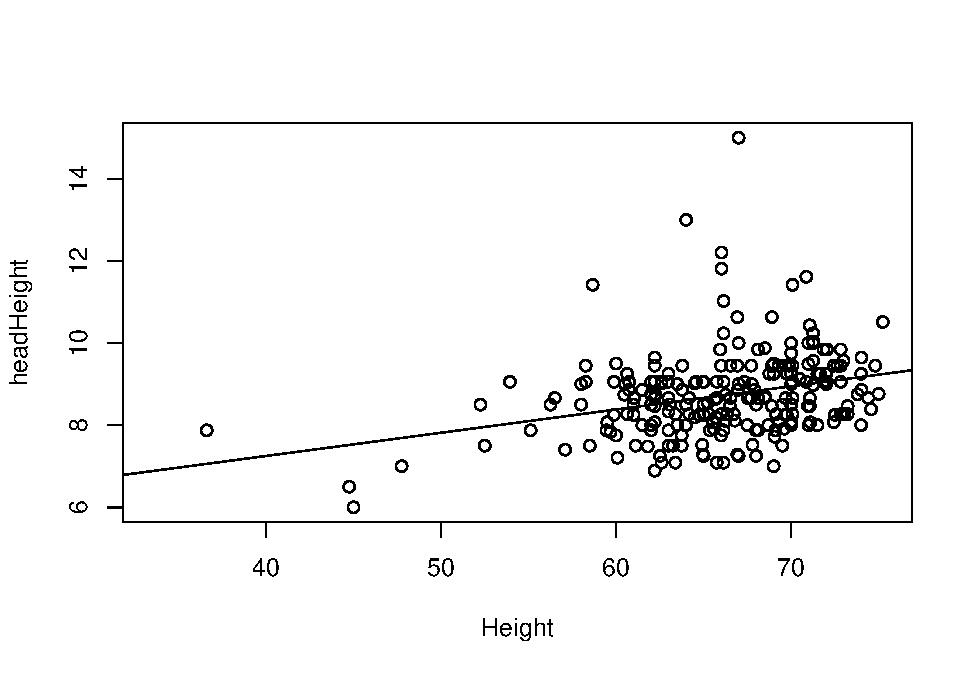
\includegraphics{project-measure-writeup_files/figure-latex/proportion-plots-1.pdf}

\begin{Shaded}
\begin{Highlighting}[]
\KeywordTok{plot}\NormalTok{(HeightAverageProportion, ArmSpanAverageProportion)}
\end{Highlighting}
\end{Shaded}

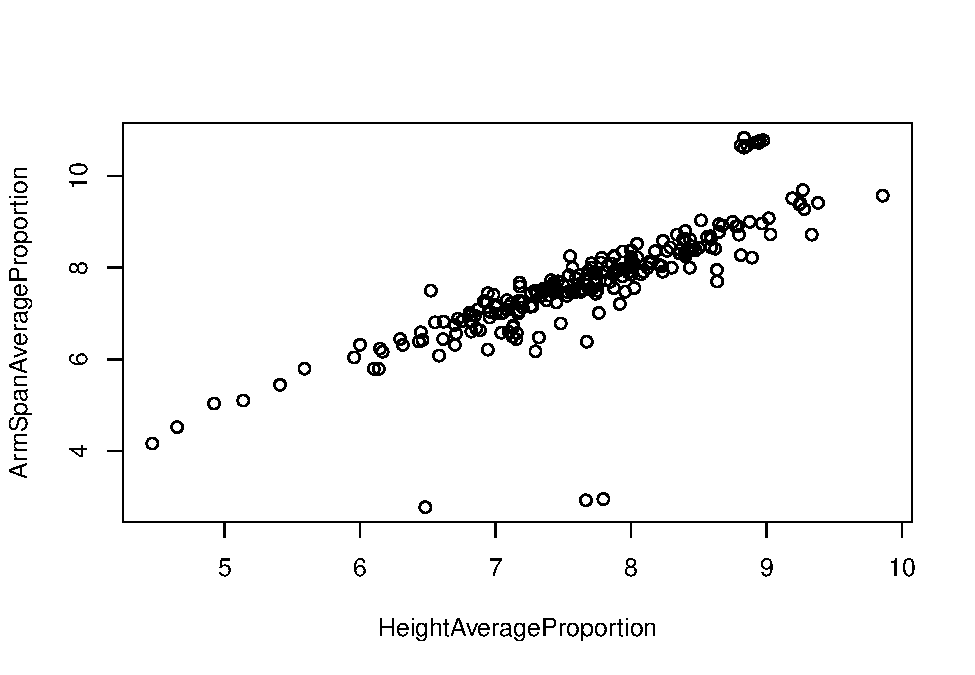
\includegraphics{project-measure-writeup_files/figure-latex/proportion-plots-2.pdf}

\begin{Shaded}
\begin{Highlighting}[]
\NormalTok{reg.n =}\StringTok{ }\KeywordTok{lm}\NormalTok{(ArmSpanAverageProportion }\OperatorTok{\textasciitilde{}}\StringTok{ }\NormalTok{HeightAverageProportion)}

\NormalTok{Strangeproportions.df =}\StringTok{ }\NormalTok{proportion.df[proportion.df}\OperatorTok{$}\NormalTok{data\_collector }\OperatorTok{==}\StringTok{ "c51267de031fb6d879a8abf25d260269"}\NormalTok{, ]}
\NormalTok{Correctproportions.df =}\StringTok{ }\NormalTok{proportion.df[proportion.df}\OperatorTok{$}\NormalTok{data\_collector }\OperatorTok{==}\StringTok{ "fd36e2b3ec59dbd996587454cbb59725"}\NormalTok{, ]}

\NormalTok{smallerProportions.df =}\StringTok{ }\NormalTok{proportion.df[proportion.df}\OperatorTok{$}\NormalTok{data\_collector }\OperatorTok{==}\StringTok{   "5a2f371a934f22dffcf1e994cb6eca40"}\NormalTok{, ]}
\NormalTok{smallerProportions1.df =}\StringTok{ }\NormalTok{smallerProportions.df[}\OperatorTok{{-}}\DecValTok{1}\NormalTok{,]}
\NormalTok{smallerProportions2.df =}\StringTok{ }\NormalTok{smallerProportions1.df[}\OperatorTok{{-}}\DecValTok{1}\NormalTok{,]}

\NormalTok{Correctproportions1.df =}\StringTok{ }\NormalTok{Correctproportions.df[}\OperatorTok{{-}}\DecValTok{1}\NormalTok{,]}

\KeywordTok{hist}\NormalTok{(Strangeproportions.df}\OperatorTok{$}\NormalTok{arm.span)}
\end{Highlighting}
\end{Shaded}

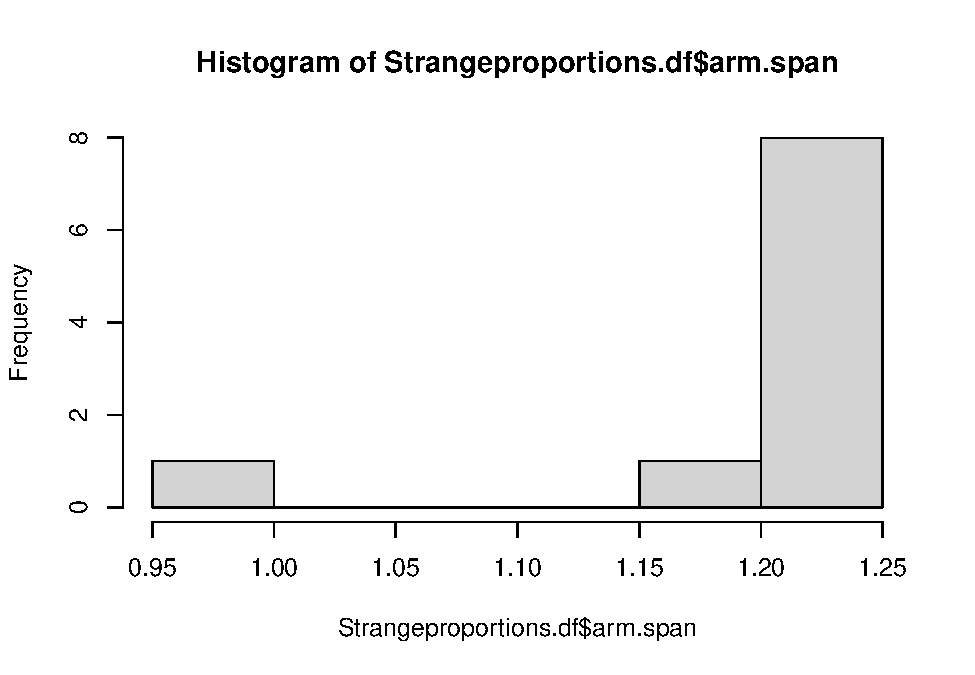
\includegraphics{project-measure-writeup_files/figure-latex/proportion-plots-3.pdf}

\begin{Shaded}
\begin{Highlighting}[]
\KeywordTok{par}\NormalTok{(}\DataTypeTok{mfrow =} \KeywordTok{c}\NormalTok{(}\DecValTok{1}\NormalTok{,}\DecValTok{2}\NormalTok{))}
\NormalTok{CorrectArmSpan =}\StringTok{ }\NormalTok{Correctproportions1.df}\OperatorTok{$}\NormalTok{arm.span}
\NormalTok{SmallArmSpan =}\StringTok{ }\NormalTok{smallerProportions2.df}\OperatorTok{$}\NormalTok{arm.span}
\KeywordTok{hist}\NormalTok{(CorrectArmSpan)}
\KeywordTok{hist}\NormalTok{(SmallArmSpan)}
\end{Highlighting}
\end{Shaded}

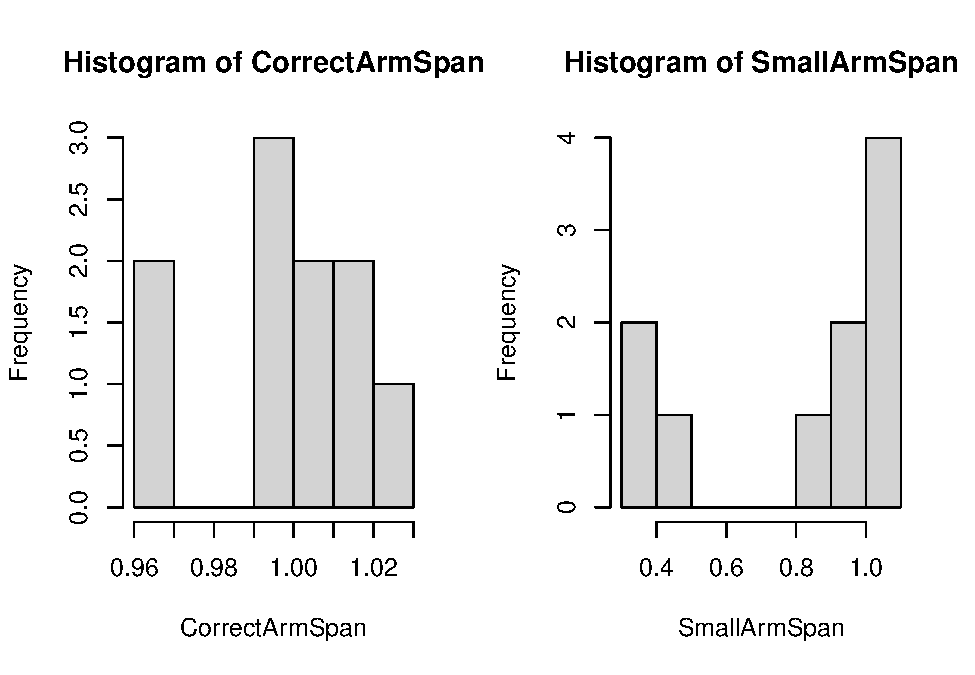
\includegraphics{project-measure-writeup_files/figure-latex/proportion-plots-4.pdf}

\begin{Shaded}
\begin{Highlighting}[]
\CommentTok{\#summary(proportion.df) removed because I show this earlier in the document}
\end{Highlighting}
\end{Shaded}

\subsection{Correlation table for Larger armspan Subset}
\label{sec:Large- correlation-tables}
\begin{sidewaystable}[!htbp]
\footnotesize
\centering
\caption{\textbf{Descriptive Statistics and Correlation Analysis}}
\label{table:correlation}
\begin{tabularx}{0.6\textwidth}{{r@{ \ \ } p{35mm} r@{}lp{1mm} r@{}l p{5mm} r@{}l p{2mm}   r@{}l  }}
 & \\
\hline
 & \\
\multicolumn{2}{c}{\textbf{ }} & \multicolumn{2}{c}{\textbf{M}} & & \multicolumn{2}{c}{\textbf{SD}} &  & \multicolumn{2}{c}{\textbf{1}} &  & \\ 
 & \\
\hline
 & \\
\textbf{1} & \textbf{Correct arm span measurements} &  1&.0 &  &  &.02 &  &  1&  &  & \\ 
 & \\
\textbf{2} & \textbf{Faulty arm span measurements} &  1&.2 &  &  &.07 &  &  &.64{$^{*}$}  &  & \\ 
 & \\
\hline
 & \\
\multicolumn{10}{p{0.54\textwidth}}{  \footnotesize { \begin{hangparas}{0.75in}{1} \textbf{\underline{Notes}:} \ \ Pearson pairwise correlations are reported; \newline a two-side test was performed to report correlation significance.  \end{hangparas} } }  & \\  
\multicolumn{10}{p{0.54\textwidth}}{  {\tiny {$^{\dagger} p < .10$} }  {     } {\tiny        {$^{*} p < .05$} }  {     } {\tiny       {$^{**} p < .01$} }  {     } {\tiny      {$^{***} p < .001$} } {     }     } & \\ 
 & \\
\hline
\end{tabularx}
\end{sidewaystable}


Below is the code to generate the summary statistics and save them as a
table that you see in Section \ref{}.

\begin{Shaded}
\begin{Highlighting}[]
\NormalTok{LargeData.df =}\StringTok{ }\NormalTok{proportion.df[proportion.df}\OperatorTok{$}\NormalTok{data\_collector }\OperatorTok{==}\StringTok{ "c51267de031fb6d879a8abf25d260269"}\NormalTok{, ]}
\NormalTok{validData.df =}\StringTok{ }\NormalTok{proportion.df[proportion.df}\OperatorTok{$}\NormalTok{data\_collector }\OperatorTok{==}\StringTok{ "fd36e2b3ec59dbd996587454cbb59725"}\NormalTok{,]}
\NormalTok{heightData1 =}\StringTok{ }\NormalTok{validData.df[}\OperatorTok{{-}}\DecValTok{1}\NormalTok{,]}
\NormalTok{helper =}\StringTok{ }\NormalTok{heightData1}\OperatorTok{$}\NormalTok{arm.span}
\NormalTok{combined2 =}\StringTok{ }\KeywordTok{data.frame}\NormalTok{(}\StringTok{"goodData"}\NormalTok{ =}\StringTok{ }\NormalTok{heightData1, }\StringTok{"badData"}\NormalTok{ =}\StringTok{ }\NormalTok{LargeData.df)}

\NormalTok{path.tables =}\StringTok{ }\KeywordTok{paste0}\NormalTok{(path.project,}\StringTok{"tables/"}\NormalTok{)}
\NormalTok{file.correlation =}\StringTok{ }\KeywordTok{paste0}\NormalTok{(path.tables,}\StringTok{"Project{-}one{-}correlation.tex"}\NormalTok{);}
\NormalTok{myData2 =}\StringTok{ }\KeywordTok{as.matrix}\NormalTok{(combined2[,}\KeywordTok{c}\NormalTok{(}\StringTok{"goodData.arm.span"}\NormalTok{, }\StringTok{"badData.arm.span"}\NormalTok{)]);  }\CommentTok{\# numeric values only, only what will appear in table}
\KeywordTok{buildLatexCorrelationTable}\NormalTok{(myData2, }
  \DataTypeTok{rotateTable =} \OtherTok{TRUE}\NormalTok{,}
  \DataTypeTok{width.table =} \FloatTok{0.60}\NormalTok{, }\CommentTok{\# best for given data ... 0.95 when rotateTable = FALSE}
                      \CommentTok{\# 0.60 when rotateTable = TRUE}
  \DataTypeTok{myFile =}\NormalTok{ file.correlation,}
  \DataTypeTok{myNames =} \KeywordTok{c}\NormalTok{(}\StringTok{"Correct arm span measurements"}\NormalTok{, }\StringTok{"Faulty arm span measurements"}\NormalTok{) );}
\KeywordTok{Sys.sleep}\NormalTok{(}\DecValTok{2}\NormalTok{); }\CommentTok{\# in case Knit{-}PDF doesn\textquotesingle{}t like that I just created the file...}
\end{Highlighting}
\end{Shaded}

\subsection{Correlation Table for Small armspan Subset}
\label{sec:Small-correlation-tables}
\begin{sidewaystable}[!htbp]
\footnotesize
\centering
\caption{\textbf{Descriptive Statistics and Correlation Analysis}}
\label{table:correlation}
\begin{tabularx}{0.6\textwidth}{{r@{ \ \ } p{35mm} r@{}lp{1mm} r@{}l p{5mm} r@{}l p{2mm}   r@{}l  }}
 & \\
\hline
 & \\
\multicolumn{2}{c}{\textbf{ }} & \multicolumn{2}{c}{\textbf{M}} & & \multicolumn{2}{c}{\textbf{SD}} &  & \multicolumn{2}{c}{\textbf{1}} &  & \\ 
 & \\
\hline
 & \\
\textbf{1} & \textbf{Correct arm span measurements} &  1&.0 &  &  &.02 &  &  1&  &  & \\ 
 & \\
\textbf{2} & \textbf{Large Faulty arm span measurements} &  &.8 &  &  &.29 &  &  -&.37 &  & \\ 
 & \\
\hline
 & \\
\multicolumn{10}{p{0.54\textwidth}}{  \footnotesize { \begin{hangparas}{0.75in}{1} \textbf{\underline{Notes}:} \ \ Pearson pairwise correlations are reported; \newline a two-side test was performed to report correlation significance.  \end{hangparas} } }  & \\  
\multicolumn{10}{p{0.54\textwidth}}{  {\tiny {$^{\dagger} p < .10$} }  {     } {\tiny        {$^{*} p < .05$} }  {     } {\tiny       {$^{**} p < .01$} }  {     } {\tiny      {$^{***} p < .001$} } {     }     } & \\ 
 & \\
\hline
\end{tabularx}
\end{sidewaystable}


\begin{Shaded}
\begin{Highlighting}[]
\NormalTok{ShortData.df =}\StringTok{ }\NormalTok{proportion.df[proportion.df}\OperatorTok{$}\NormalTok{data\_collector }\OperatorTok{==}\StringTok{ "5a2f371a934f22dffcf1e994cb6eca40"}\NormalTok{, ]}

\NormalTok{heightData.df =}\StringTok{ }\NormalTok{proportion.df[proportion.df}\OperatorTok{$}\NormalTok{data\_collector }\OperatorTok{==}\StringTok{ "fd36e2b3ec59dbd996587454cbb59725"}\NormalTok{,]}
\NormalTok{heightData2 =}\StringTok{ }\NormalTok{heightData.df[}\OperatorTok{{-}}\DecValTok{1}\NormalTok{,]}
\NormalTok{ShortDataFix =}\StringTok{ }\NormalTok{ShortData.df[}\OperatorTok{{-}}\DecValTok{3}\NormalTok{, ]}
\NormalTok{ShortDataFix1 =}\StringTok{ }\NormalTok{ShortDataFix[}\OperatorTok{{-}}\DecValTok{4}\NormalTok{, ]}
\NormalTok{helper =}\StringTok{ }\NormalTok{heightData1}\OperatorTok{$}\NormalTok{arm.span}
\NormalTok{combined =}\StringTok{ }\KeywordTok{data.frame}\NormalTok{(}\StringTok{"goodData"}\NormalTok{ =}\StringTok{ }\NormalTok{heightData2, }\StringTok{"badData"}\NormalTok{ =}\StringTok{ }\NormalTok{ShortDataFix1)}

\NormalTok{path.tables =}\StringTok{ }\KeywordTok{paste0}\NormalTok{(path.project,}\StringTok{"tables/"}\NormalTok{)}
\NormalTok{file.correlation =}\StringTok{ }\KeywordTok{paste0}\NormalTok{(path.tables,}\StringTok{"Project{-}one{-}correlation{-}table.tex"}\NormalTok{);}
\NormalTok{myData =}\StringTok{ }\KeywordTok{as.matrix}\NormalTok{(combined[,}\KeywordTok{c}\NormalTok{(}\StringTok{"goodData.arm.span"}\NormalTok{, }\StringTok{"badData.arm.span"}\NormalTok{)]);  }\CommentTok{\# numeric values only, only what will appear in table}

\KeywordTok{buildLatexCorrelationTable}\NormalTok{(myData, }
  \DataTypeTok{rotateTable =} \OtherTok{TRUE}\NormalTok{,}
  \DataTypeTok{width.table =} \FloatTok{0.60}\NormalTok{, }\CommentTok{\# best for given data ... 0.95 when rotateTable = FALSE}
                      \CommentTok{\# 0.60 when rotateTable = TRUE}
  \DataTypeTok{myFile =}\NormalTok{ file.correlation,}
  \DataTypeTok{myNames =} \KeywordTok{c}\NormalTok{(}\StringTok{"Correct arm span measurements"}\NormalTok{, }\StringTok{"Large Faulty arm span measurements"}\NormalTok{) );}
\KeywordTok{Sys.sleep}\NormalTok{(}\DecValTok{2}\NormalTok{); }\CommentTok{\# in case Knit{-}PDF doesn\textquotesingle{}t like that I just created the file...}
\end{Highlighting}
\end{Shaded}

\subsection{Welch T-Tests}

\begin{Shaded}
\begin{Highlighting}[]
\NormalTok{  StrangeData.df =}\StringTok{ }\NormalTok{proportion.df[proportion.df}\OperatorTok{$}\NormalTok{data\_collector }\OperatorTok{==}\StringTok{ "c51267de031fb6d879a8abf25d260269"}\NormalTok{, ]}
\NormalTok{  StrangerData.df =}\StringTok{ }\NormalTok{StrangeData.df}\OperatorTok{$}\NormalTok{arm.span}
\NormalTok{  heightData.df =}\StringTok{ }\NormalTok{proportion.df[proportion.df}\OperatorTok{$}\NormalTok{data\_collector }\OperatorTok{==}\StringTok{ "fd36e2b3ec59dbd996587454cbb59725"}\NormalTok{,]}
\NormalTok{  heightData1 =}\StringTok{ }\NormalTok{heightData.df[}\OperatorTok{{-}}\DecValTok{1}\NormalTok{,]}
\NormalTok{  try=}\StringTok{ }\KeywordTok{round}\NormalTok{(StrangerData.df, }\DataTypeTok{digits =} \DecValTok{3}\NormalTok{)}
\NormalTok{  helper =}\StringTok{ }\NormalTok{heightData1}\OperatorTok{$}\NormalTok{arm.span}
\NormalTok{  combined =}\StringTok{ }\KeywordTok{data.frame}\NormalTok{(}\StringTok{"goodData"}\NormalTok{ =}\StringTok{ }\NormalTok{helper, }\StringTok{"badData"}\NormalTok{ =}\StringTok{ }\NormalTok{try)}
  
\NormalTok{  proportions1.df =}\StringTok{ }\NormalTok{proportion.df[proportion.df}\OperatorTok{$}\NormalTok{data\_collector }\OperatorTok{!=}\StringTok{ "c51267de031fb6d879a8abf25d260269"}\NormalTok{, ]}
  
\NormalTok{  CorrectArmSpan =}\StringTok{ }\NormalTok{proportions1.df}\OperatorTok{$}\NormalTok{arm.span}
\NormalTok{  IncorrectArmSpan =}\StringTok{ }\NormalTok{combined}\OperatorTok{$}\NormalTok{badData}
  
  \KeywordTok{t.test}\NormalTok{(CorrectArmSpan, IncorrectArmSpan)}
\end{Highlighting}
\end{Shaded}

\begin{verbatim}
## 
##  Welch Two Sample t-test
## 
## data:  CorrectArmSpan and IncorrectArmSpan
## t = -8.5806, df = 10.062, p-value = 6.086e-06
## alternative hypothesis: true difference in means is not equal to 0
## 95 percent confidence interval:
##  -0.2424512 -0.1425588
## sample estimates:
## mean of x mean of y 
##  0.991595  1.184100
\end{verbatim}

\begin{Shaded}
\begin{Highlighting}[]
\NormalTok{  StrangeData.df =}\StringTok{ }\NormalTok{proportion.df[proportion.df}\OperatorTok{$}\NormalTok{data\_collector }\OperatorTok{==}\StringTok{ "5a2f371a934f22dffcf1e994cb6eca40"}\NormalTok{, ]}
\NormalTok{  StrangeData1.df =}\StringTok{ }\NormalTok{StrangeData.df[}\OperatorTok{{-}}\DecValTok{1}\NormalTok{,]}
\NormalTok{  StrangeData2.df =}\StringTok{ }\NormalTok{StrangeData1.df[}\OperatorTok{{-}}\DecValTok{4}\NormalTok{,]}
\NormalTok{  StrangerData.df =}\StringTok{ }\NormalTok{StrangeData2.df}\OperatorTok{$}\NormalTok{arm.span}
  
\NormalTok{  heightData.df =}\StringTok{ }\NormalTok{proportion.df[proportion.df}\OperatorTok{$}\NormalTok{data\_collector }\OperatorTok{==}\StringTok{ "fd36e2b3ec59dbd996587454cbb59725"}\NormalTok{,]}
\NormalTok{  heightData1 =}\StringTok{ }\NormalTok{heightData.df[}\OperatorTok{{-}}\DecValTok{1}\NormalTok{,]}
\NormalTok{  try=}\StringTok{ }\KeywordTok{round}\NormalTok{(StrangerData.df, }\DataTypeTok{digits =} \DecValTok{3}\NormalTok{)}
\NormalTok{  helper =}\StringTok{ }\KeywordTok{round}\NormalTok{(heightData1}\OperatorTok{$}\NormalTok{arm.span, }\DataTypeTok{digits =} \DecValTok{3}\NormalTok{)}
\NormalTok{  combined2 =}\StringTok{ }\KeywordTok{data.frame}\NormalTok{(}\StringTok{"goodData"}\NormalTok{ =}\StringTok{ }\NormalTok{helper, }\StringTok{"badData"}\NormalTok{ =}\StringTok{ }\NormalTok{try)}
  
\NormalTok{  proportions2.df =}\StringTok{ }\NormalTok{proportion.df[proportion.df}\OperatorTok{$}\NormalTok{data\_collector }\OperatorTok{!=}\StringTok{ "5a2f371a934f22dffcf1e994cb6eca40"}\NormalTok{, ]}
  
\NormalTok{  CorrectArmSpan =}\StringTok{ }\NormalTok{proportions2.df}\OperatorTok{$}\NormalTok{arm.span}
\NormalTok{  IncorrectArmSpan =}\StringTok{ }\NormalTok{combined2}\OperatorTok{$}\NormalTok{badData}
  
  \KeywordTok{t.test}\NormalTok{(CorrectArmSpan, IncorrectArmSpan)}
\end{Highlighting}
\end{Shaded}

\begin{verbatim}
## 
##  Welch Two Sample t-test
## 
## data:  CorrectArmSpan and IncorrectArmSpan
## t = 2.1027, df = 9.0295, p-value = 0.06473
## alternative hypothesis: true difference in means is not equal to 0
## 95 percent confidence interval:
##  -0.0145928  0.4023104
## sample estimates:
## mean of x mean of y 
##  1.007859  0.814000
\end{verbatim}

\subsection{Final Histograms}

\begin{Shaded}
\begin{Highlighting}[]
\NormalTok{proportionHist.df =}\StringTok{ }\NormalTok{measure.df}

\NormalTok{proportionHist1.df =}\StringTok{ }\NormalTok{proportionHist.df[proportionHist.df}\OperatorTok{$}\NormalTok{data\_collector }\OperatorTok{!=}\StringTok{ "c51267de031fb6d879a8abf25d260269"}\NormalTok{, ]}


\NormalTok{StrangeData.df =}\StringTok{ }\NormalTok{measure.df[measure.df}\OperatorTok{$}\NormalTok{data\_collector }\OperatorTok{==}\StringTok{ "c51267de031fb6d879a8abf25d260269"}\NormalTok{, ]}
\NormalTok{MonkeyData.df =}\StringTok{ }\NormalTok{StrangeData.df}\OperatorTok{$}\NormalTok{arm.span}
\KeywordTok{par}\NormalTok{(}\DataTypeTok{mfrow =} \KeywordTok{c}\NormalTok{(}\DecValTok{1}\NormalTok{,}\DecValTok{2}\NormalTok{))}
\KeywordTok{hist}\NormalTok{(MonkeyData.df, }\DataTypeTok{main =} \StringTok{"Histogram of data anomaly"}\NormalTok{)}
\NormalTok{heightData =}\StringTok{ }\NormalTok{proportionHist1.df}\OperatorTok{$}\NormalTok{arm.span}
\KeywordTok{hist}\NormalTok{(heightData, }\DataTypeTok{main =} \StringTok{"Without the anomaly"}\NormalTok{)}
\end{Highlighting}
\end{Shaded}

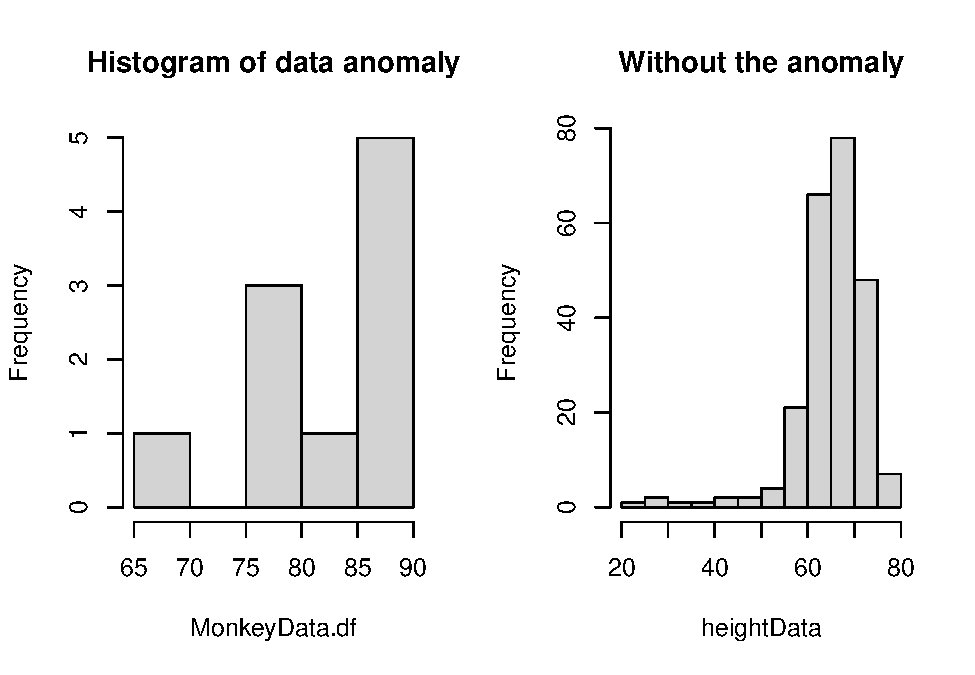
\includegraphics{project-measure-writeup_files/figure-latex/histogram-1.pdf}




%% appendices go here!


\newpage
\theendnotes

%%%%%%%%%%%%%%%%%%%%%%%%%%%%%%%%%%%  biblio %%%%%%%%
\newpage
\begin{auxmulticols}{2}
\singlespacing 
\bibliography{./../biblio/master.bib}

%%%%%%%%%%%%%%%%%%%%%%%%%%%%%%%%%%%  biblio %%%%%%%%
\end{auxmulticols}

\newpage
{
\hypersetup{linkcolor=black}
\setcounter{tocdepth}{3}
\tableofcontents
}



\end{document}